% Conceptual schematic for the composition gap pipeline.
% Compile standalone: pdflatex fig_schematic.tex
\documentclass[tikz,border=8pt]{standalone}
\usepackage{amsmath,amssymb}
\usetikzlibrary{arrows.meta,positioning,calc}

\definecolor{boxblue}{HTML}{DBEAFE}
\definecolor{bordblue}{HTML}{3B82F6}
\definecolor{boxorange}{HTML}{FEF3C7}
\definecolor{bordorange}{HTML}{D97706}
\definecolor{boxgreen}{HTML}{D1FAE5}
\definecolor{bordgreen}{HTML}{059669}
\definecolor{boxpurple}{HTML}{EDE9FE}
\definecolor{bordpurple}{HTML}{7C3AED}
\definecolor{anncolor}{HTML}{6B7280}

\begin{document}
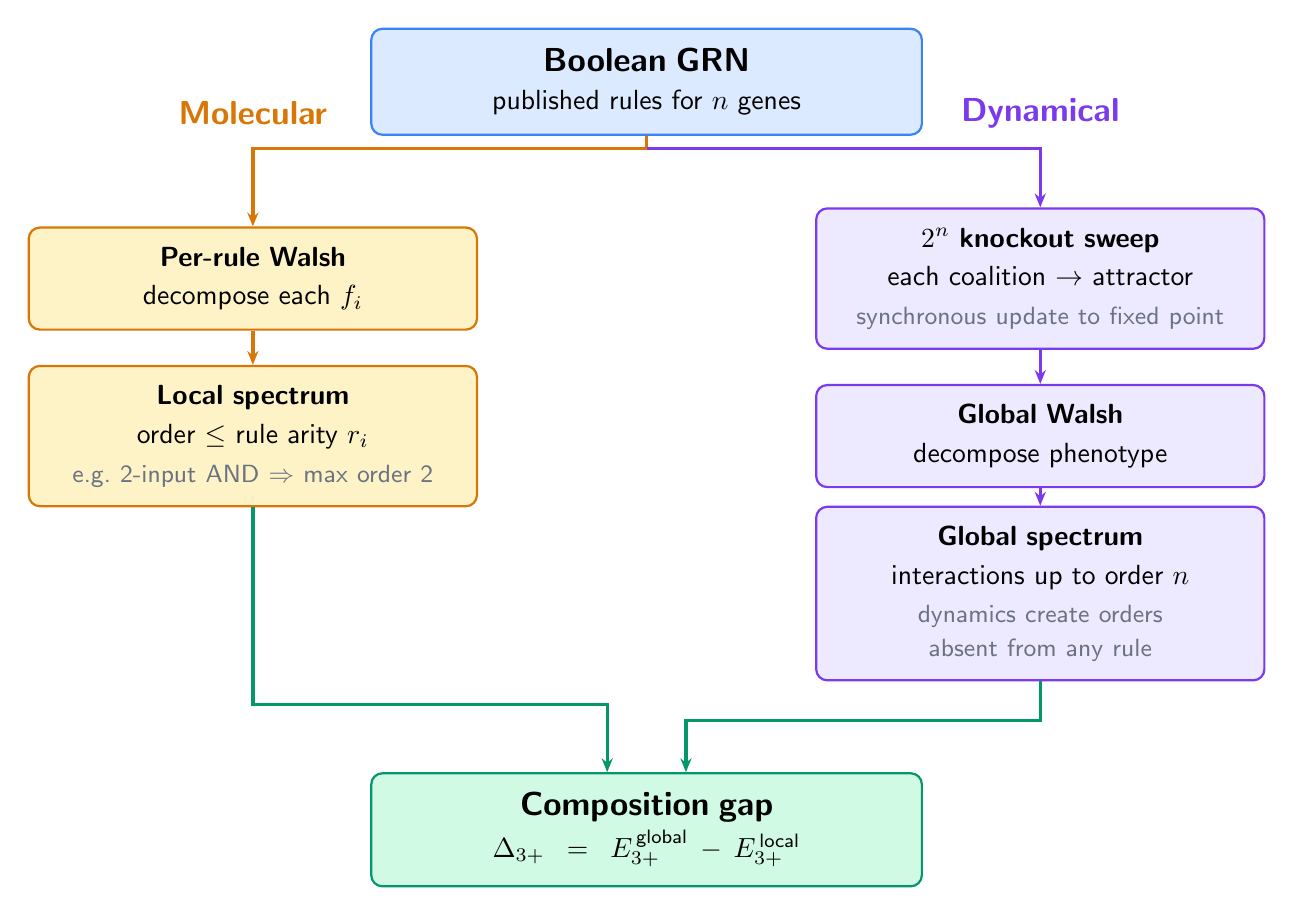
\begin{tikzpicture}[
    box/.style={
        rectangle, rounded corners=4pt,
        text centered, font=\sffamily,
        line width=0.8pt, inner sep=7pt,
        text width=5.2cm,
    },
    mainbox/.style={box, draw=bordblue, fill=boxblue, text width=6.5cm},
    localbox/.style={box, draw=bordorange, fill=boxorange},
    globalbox/.style={box, draw=bordpurple, fill=boxpurple},
    resultbox/.style={box, draw=bordgreen, fill=boxgreen, text width=6.5cm},
    arr/.style={-{Stealth[length=5pt,width=4pt]}, line width=1.2pt, color=#1},
    pathlabel/.style={font=\sffamily\large\bfseries},
]

% Wide layout: large horizontal separation, compact vertical
\def\pathsep{5.0cm}

% Top: Boolean GRN
\node[mainbox] (grn) at (0,0)
    {\textbf{\large Boolean GRN}\\[2pt]
     published rules for $n$ genes};

% Path labels — above the fork wires
\node[pathlabel, text=bordorange] at (-\pathsep,-0.4) {Molecular};
\node[pathlabel, text=bordpurple] at (\pathsep,-0.4) {Dynamical};

% Left path: Local analysis — 2 boxes closer together
\node[localbox] (local_walsh) at (-\pathsep,-2.5)
    {\textbf{Per-rule Walsh}\\[2pt]
     decompose each $f_i$};

\node[localbox] (local_spec) at (-\pathsep,-4.5)
    {\textbf{Local spectrum}\\[2pt]
     order $\leq$ rule arity $r_i$\\[2pt]
     {\small\color{anncolor} e.g.\ 2-input AND $\Rightarrow$ max order 2}};

% Right path: Global analysis — 3 boxes, tighter spacing
\node[globalbox] (sweep) at (\pathsep,-2.5)
    {\textbf{$2^n$ knockout sweep}\\[2pt]
     each coalition $\to$ attractor\\[2pt]
     {\small\color{anncolor} synchronous update to fixed point}};

\node[globalbox] (global_walsh) at (\pathsep,-4.5)
    {\textbf{Global Walsh}\\[2pt]
     decompose phenotype};

\node[globalbox] (global_spec) at (\pathsep,-6.5)
    {\textbf{Global spectrum}\\[2pt]
     interactions up to order $n$\\[2pt]
     {\small\color{anncolor} dynamics create orders absent from any rule}};

% Bottom: Composition gap — centered, extra vertical space
\node[resultbox] (gap) at (0,-9.5)
    {\textbf{\large Composition gap}\\[3pt]
     $\Delta_{3+} = E_{3+}^{\,\text{global}} - E_{3+}^{\,\text{local}}$};

% Arrows — fork from GRN
\coordinate (fork) at (0,-0.85);
\draw[arr=bordorange] (grn.south) -- (fork) -| (local_walsh.north);
\draw[arr=bordpurple] (fork) -| (sweep.north);

% Arrows — local path
\draw[arr=bordorange] (local_walsh) -- (local_spec);

% Arrows — global path
\draw[arr=bordpurple] (sweep) -- (global_walsh);
\draw[arr=bordpurple] (global_walsh) -- (global_spec);

% Arrows — converge to gap (left drops to same Y as right elbow)
\draw[arr=bordgreen] (local_spec.south) -- ++(0,-2.5) -|
    ([xshift=-0.5cm]gap.north);
\draw[arr=bordgreen] (global_spec.south) -- ++(0,-0.5) -|
    ([xshift=0.5cm]gap.north);

\end{tikzpicture}
\end{document}
